\section{Feinentwurf}
\subsection{Vorüberlegungen}
Im Zuge der Erstellung des Feinentwurfs wird das Analysemodell des Grobentwurfs in fachlicher Hinsicher vervollständigt. Üblicherweise erfolgt dies durch Definition von Klassen, Attributen, Operationen und Assoziationen in einem Klassendiagramm. Das Self-Service-Terminal wird jedoch als Webapplikation in einem gesetzten Framework entwickelt und muss daher besonderen Anforderungen genügen.
Das Django Framework trennt Datenverarbeitung, Websitedesign und Logik voneinander, damit diese Elemente möglichst unabhängig von einander entwickelt werden können. Aufgrund dessen erscheint es sinnvoll den Feinentwurf nach der Struktur des Model-Template-View-Prinzips zu entwickeln. Struktur und Aufbau der MTV-Architektur sowie die Zusammenhänge der Elemente untereinander werden in \ref{fig:MVT_Erweitert} visualisiert.

\subsection{Model-Template-View-Prinzip}
Das Model-Template-View-Prinzip basiert auf einer möglichst losen Kopplung der Softwareelemente Model, Template und View. Die Aufgaben der entsprechenden Elemente unterscheiden sich dabei naturgemäß voneinander:\par 
\vspace{0,5cm}
\noindent \textbf{Models:} \par
\vspace{0,5cm}
\noindent Durch Models wird die Datenverarbeitung der Webapplikation gesteuert. Grundsätzlich gilt, dass jede Klasse der Models einer Relation in der zugrundeliegenden Datenbank entspricht. Die erstellten Klassen sind dabei Pythen Unterklassen der Klasse \textit{django.db.models.Model}. Aus den Menu Klassen können Objekte instanziiert werden. Die Attribute der generierten Klassen entsprechen dabei den Attributen der jeweiligen Relation. Zusammen ergeben sie also das Relationsschema. Anhand dieser Informationen steuert Django Anfragen an die Datenbank mithilfe der \textit{database-access API} automatisch.\par
\vspace{0,5cm}
\noindent \textbf{Templates:}\par
\vspace{0,5cm}
\noindent Djangos Templates enthalten Informationen über die Ausgabe statischer und dynamischer HTML Elemente. Mithilfe der Django-Templatesprache ist es außerdem möglich Inhalte in Blocks aufzuteilen und diese dynamischen Inhalte aufzurufen. Django nutzt eine eigene Schnittstelle zum laden und rendern der Templates.

\newpage

\noindent \textbf{Views:}\par
\vspace{0,5cm}
\noindent Views sind Funktionen, welche eine http-Request übergeben bekommen und eine http-Response zurückgeben. Das View enthält dabei die dazu notwendige Logik. Um die Projektstruktur möglichst einfach zu halten, legen wir auch andere anwendungsbezogene Logik in der view.py Datei ab. Nur Funktionen, die direkt mit den Model-Klassen interagieren werden in der model.py abgelegt.\par
\vspace{1cm}
\begin{figure}[htp]
    \centering
    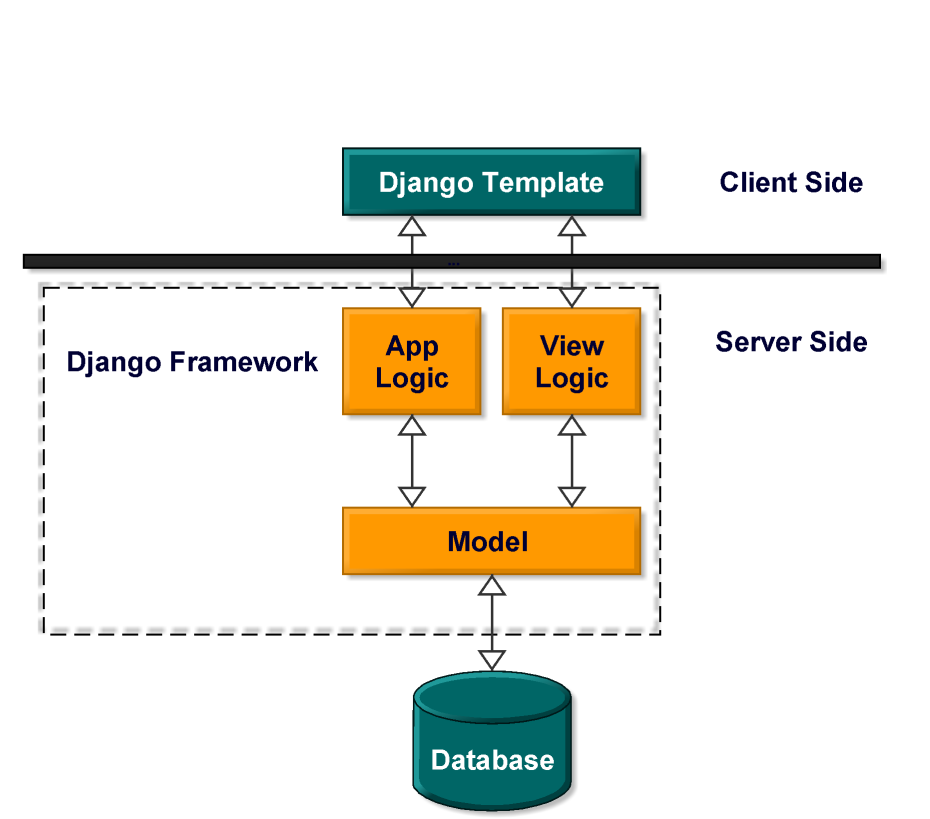
\includegraphics[width=12cm , height=11cm]{Kapitel/Bilder/MVT-Erweitert-Diesmalwirklich.PNG}
    \caption{Visualisierung des MVT-Prinzips im Django Framework}
    \label{fig:MVT_Erweitert}
\end{figure}
\newpage
\subsection{Architektur Entwurf}
Die Entwicklung des SST wird iterativ durchgeführt und orientiert sich an den zu erfüllenden Anforderungen. Die Architektur des Systems entwickelt sich daher im Geiste des gewählten agilen Vorgehensmodells Stück für Stück mit den implementierten Anforderungen. Das MTV-Prinzip gibt dabei die Struktur vor. 


